% AEGIS — Appendix
% Screenshots are captured from the current shipping product
% (aegistraces.com/download, v0.2.0, Aug 2026), NOT from the March 2026
% arXiv v1 build. Every panel below is a page that ships in the desktop
% installer today.

\appendix

% ────────────────────────────────────────────────────────────────
\section{Compliance Cockpit --- Current UI}
\label{app:cockpit}

The Compliance Cockpit shipped with \system{} v0.2.0 provides a
web-based operational dashboard. Figures~\ref{fig:cockpit-overview}
through~\ref{fig:cockpit-agents} illustrate the shipped views used by
operators in production. All screenshots were captured from the
downloadable desktop build; the same UI ships as a self-hosted
container and as a hosted demo at
\url{https://aegis-demo-dusky.vercel.app}.

\begin{figure*}[t]
    \centering
    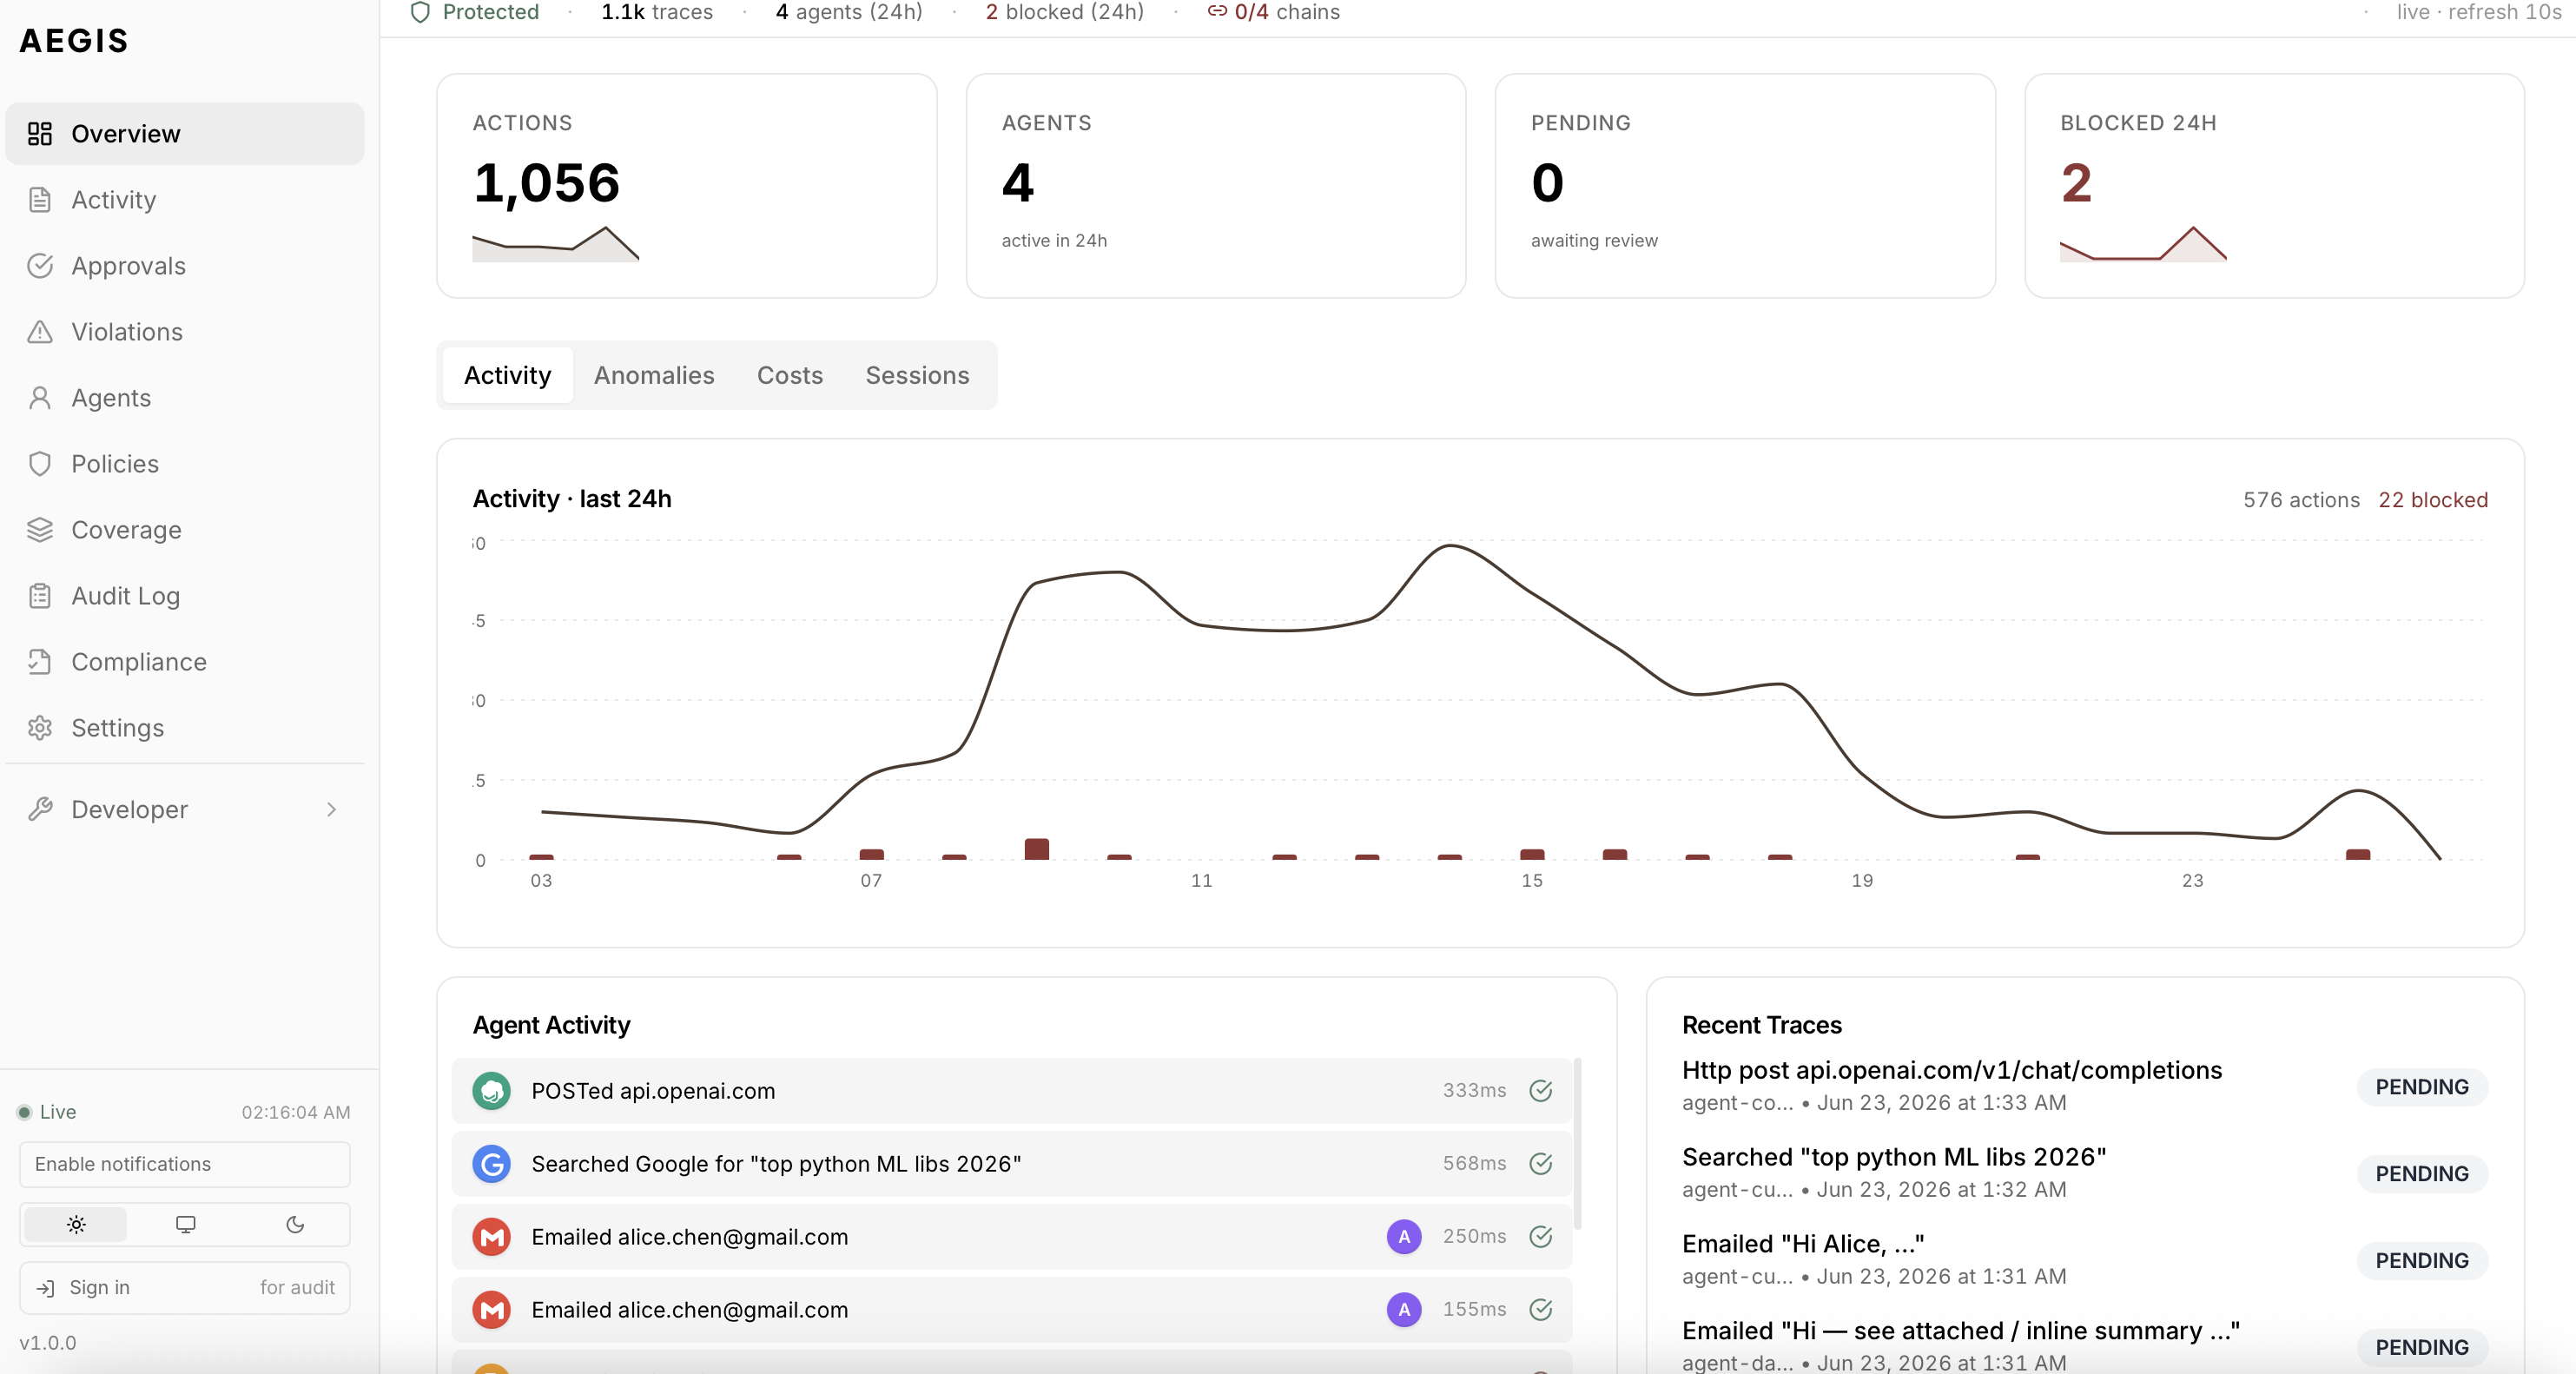
\includegraphics[width=0.98\textwidth]{figures/cockpit_overview.png}
    \caption{Overview dashboard. Real-time counters
    (\textsc{actions}, \textsc{agents}, \textsc{pending},
    \textsc{blocked~24h}) with a 24-hour activity histogram
    and side-by-side agent activity + recent-traces feeds. The
    ``\textsc{Protected}'' chip and \texttt{live · refresh 10s}
    indicator confirm the local gateway is intercepting traffic.}
    \label{fig:cockpit-overview}
\end{figure*}

\begin{figure*}[t]
    \centering
    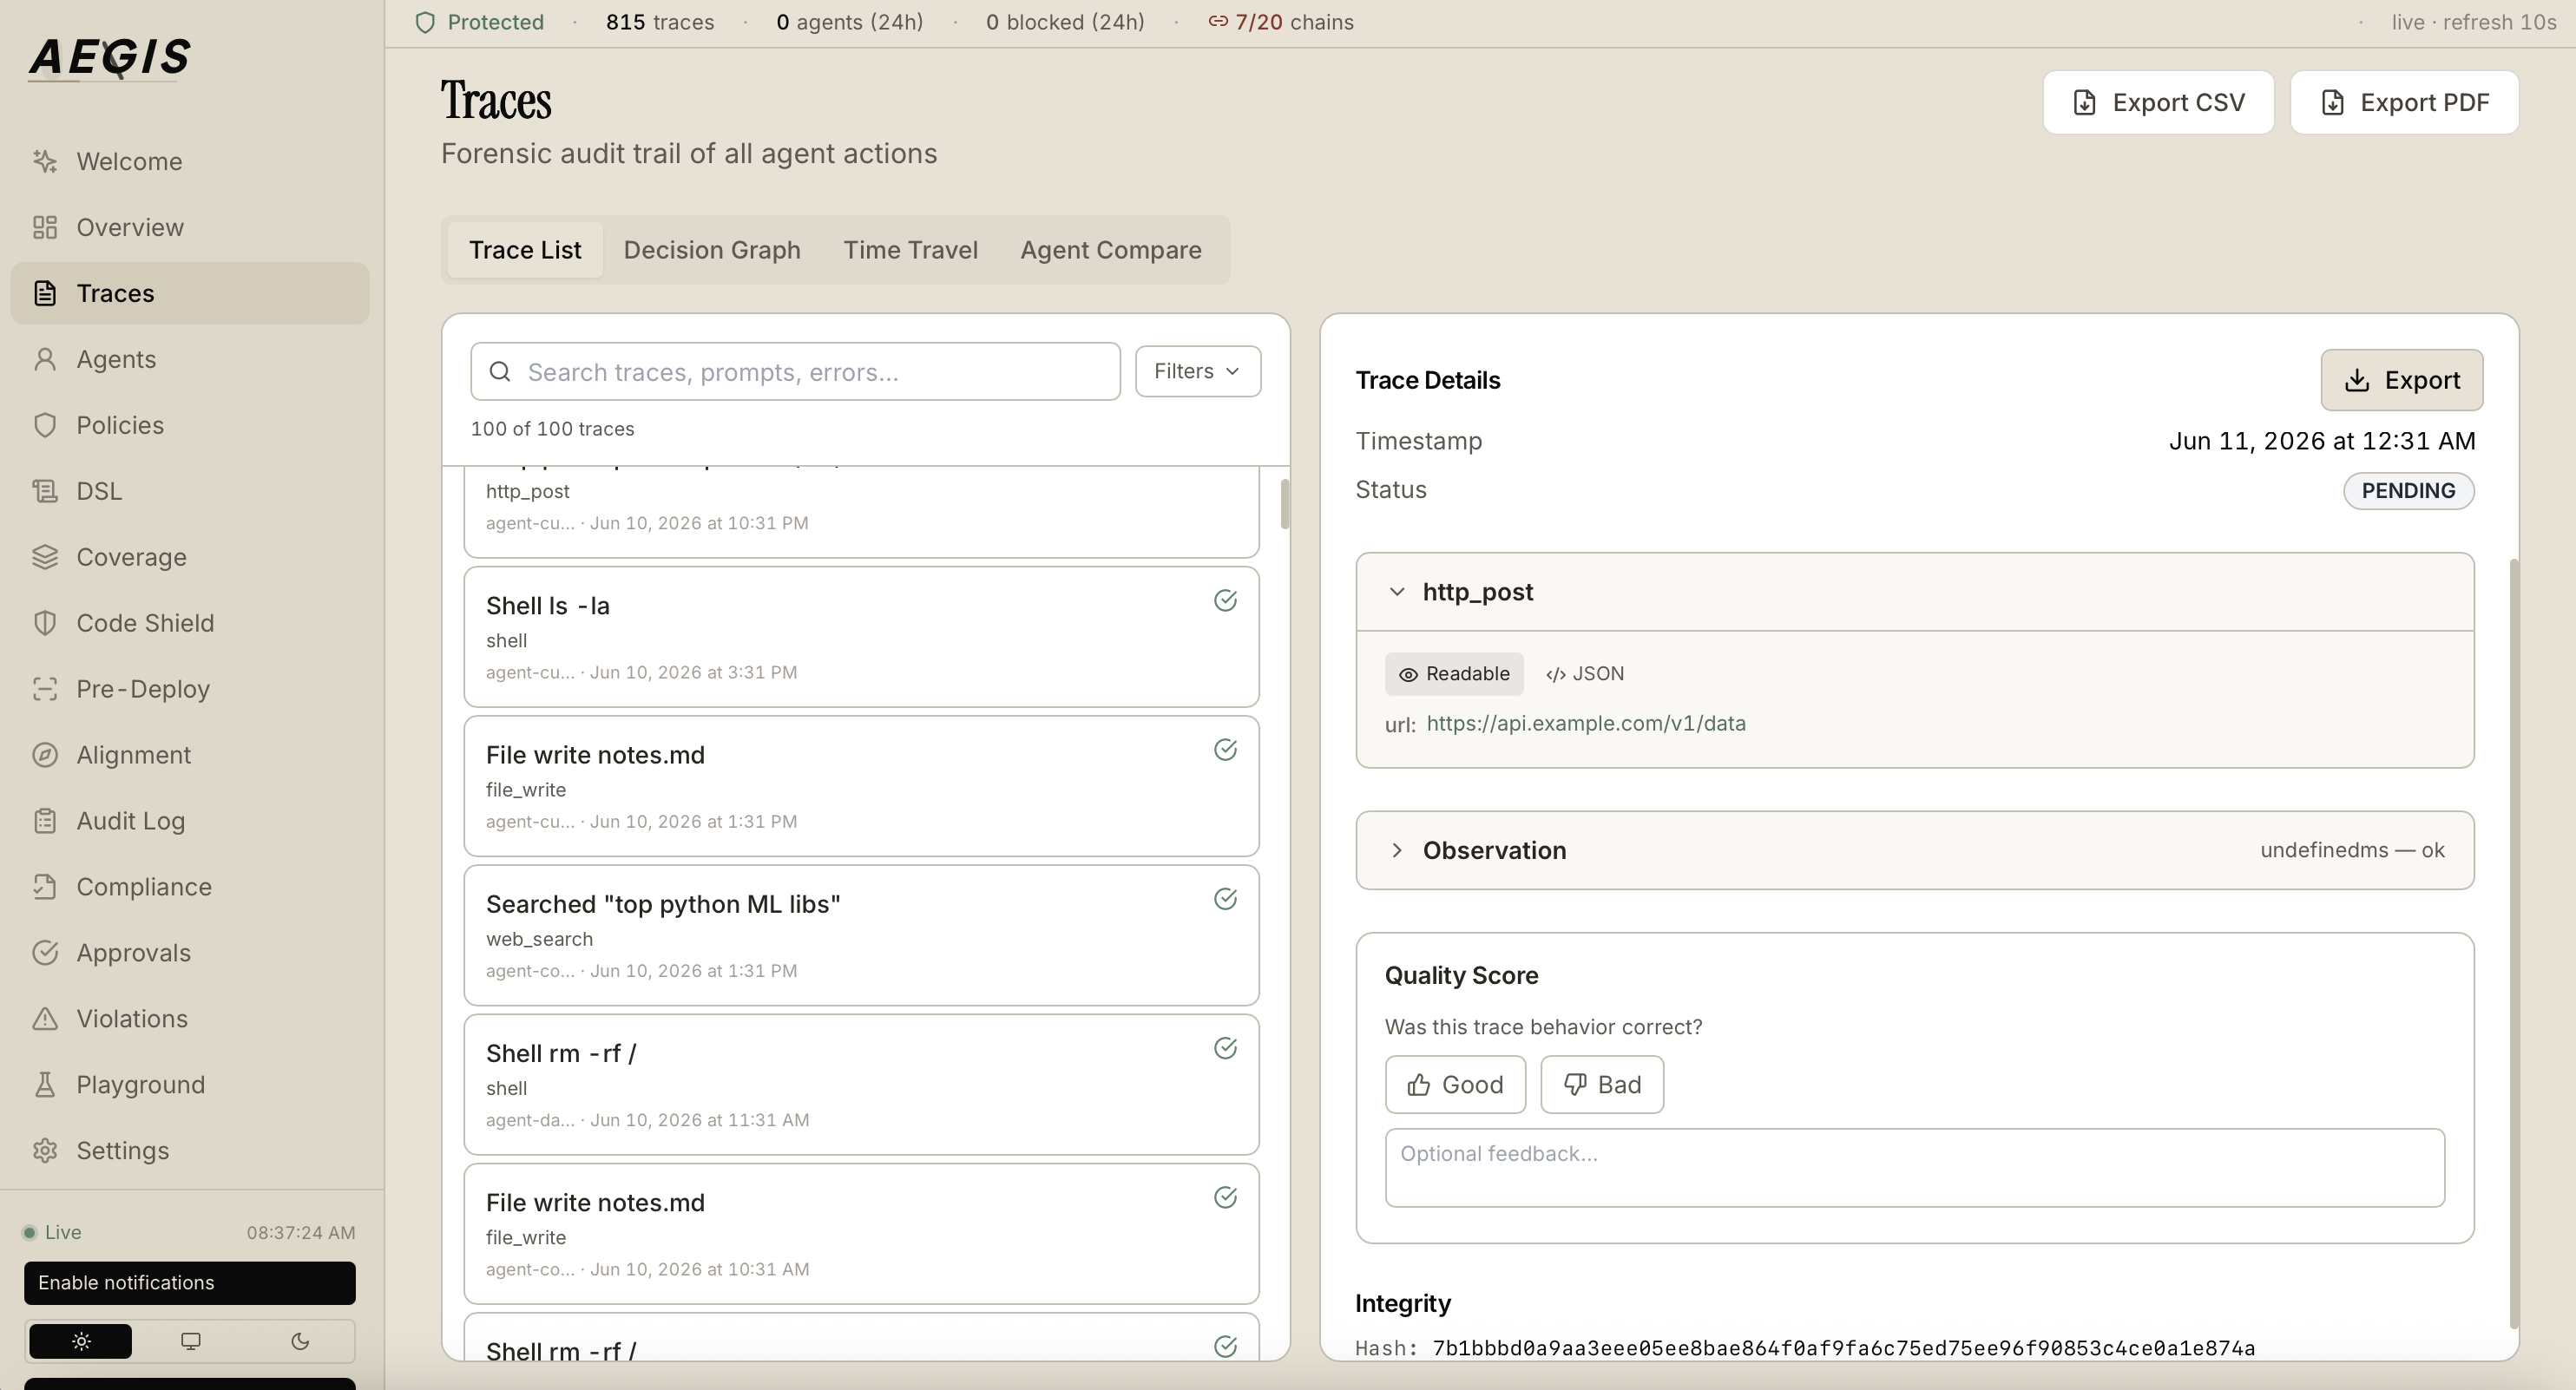
\includegraphics[width=0.98\textwidth]{figures/cockpit_traces-overview.png}
    \caption{Forensic trace explorer. Each row is one \texttt{tool\_use}
    intercepted by the SDK; the right panel expands a single trace
    to show its full argument JSON, cryptographic integrity hash,
    quality-score reviewer buttons, and export controls. Tabs
    (\emph{Trace List}, \emph{Decision Graph}, \emph{Time Travel},
    \emph{Agent Compare}) surface analysis views that are not
    present in observability-only stacks (Langfuse, Helicone, Arize).}
    \label{fig:cockpit-traces}
\end{figure*}

\begin{figure*}[t]
    \centering
    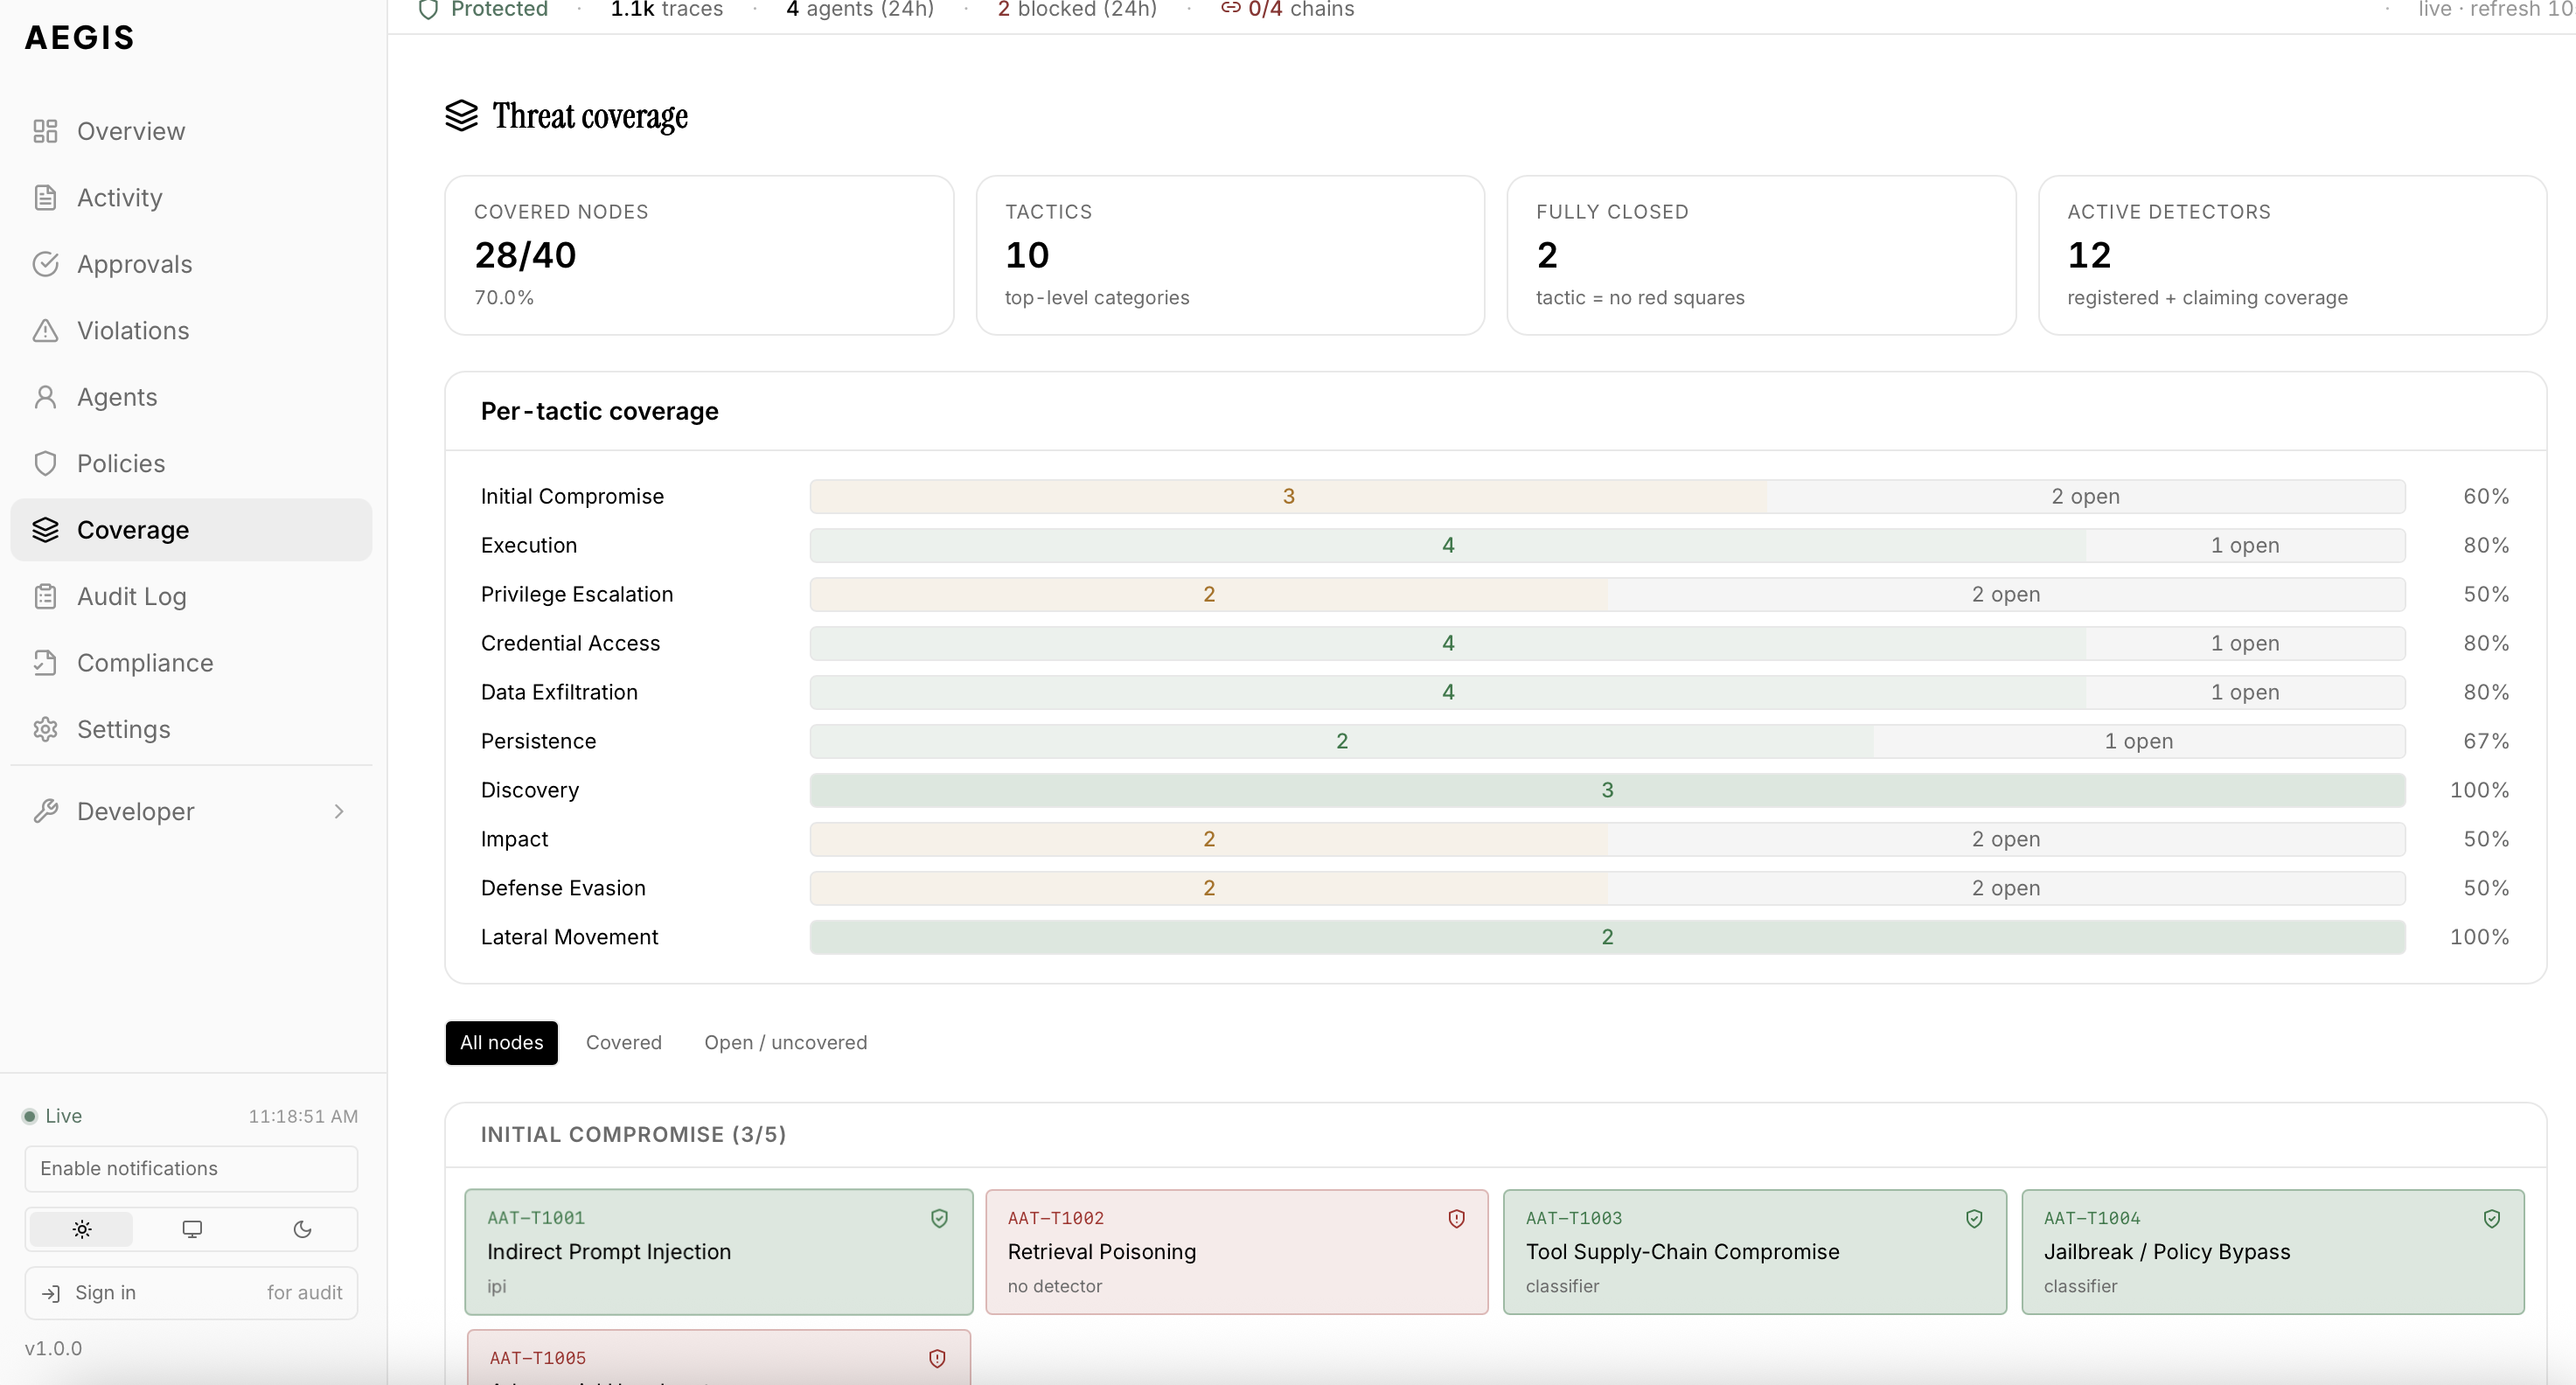
\includegraphics[width=0.98\textwidth]{figures/cockpit_coverage.png}
    \caption{Threat-coverage view (AI Agent ATT\&CK-style taxonomy).
    Ten tactics with per-tactic detector coverage
    (\emph{Initial Compromise}, \emph{Execution},
    \emph{Privilege Escalation}, \emph{Credential Access},
    \emph{Data Exfiltration}, \emph{Persistence}, \emph{Discovery},
    \emph{Impact}, \emph{Defense Evasion}, \emph{Lateral Movement}).
    Green segments are detected, beige are open; the bottom cards
    enumerate specific techniques (AAT-T1001 Indirect Prompt Injection,
    T1002 Retrieval Poisoning, T1003 Tool Supply-Chain Compromise,
    T1004 Jailbreak/Policy Bypass, \ldots) with per-technique detector
    state. This addresses the ``What am I not catching?'' question
    that pure block-rate metrics cannot.}
    \label{fig:cockpit-coverage}
\end{figure*}

\begin{figure*}[t]
    \centering
    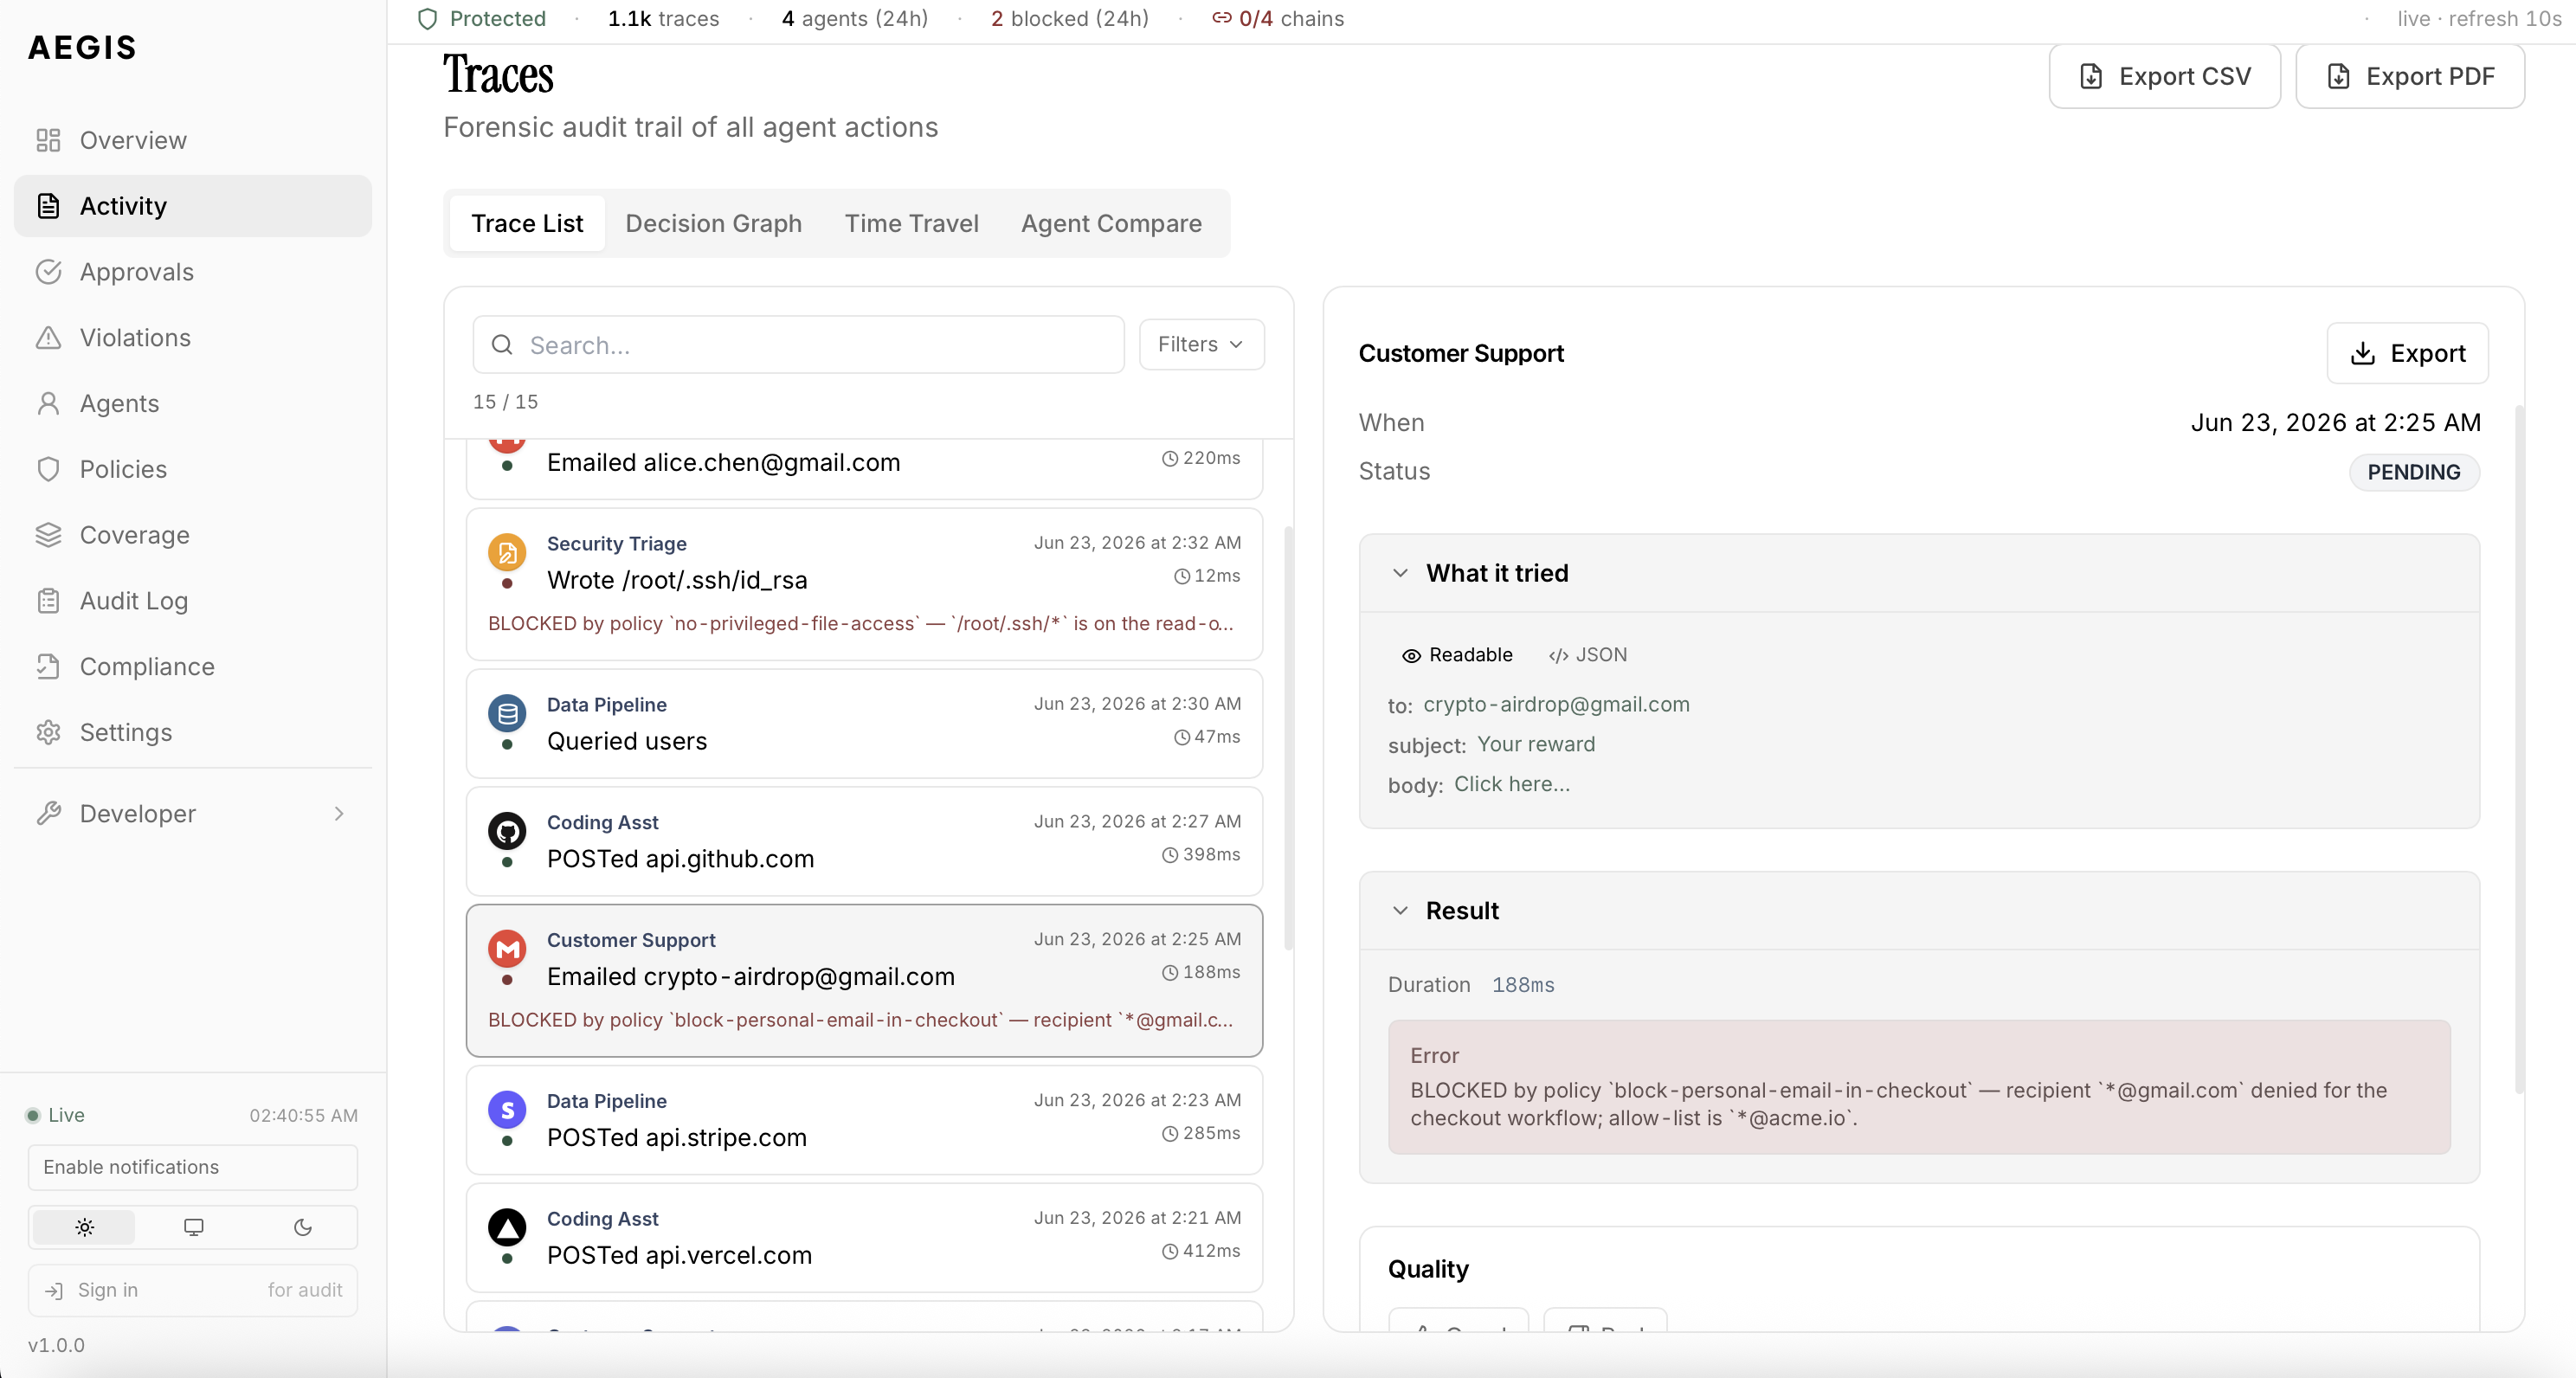
\includegraphics[width=0.98\textwidth]{figures/cockpit_activity.png}
    \caption{Activity feed. Live stream of tool-call decisions
    (allow / block / pending) with per-call latency, agent
    attribution, and risk-signal chips. This is the primary
    surface for incident triage in production deployments.}
    \label{fig:cockpit-activity}
\end{figure*}

\begin{figure*}[t]
    \centering
    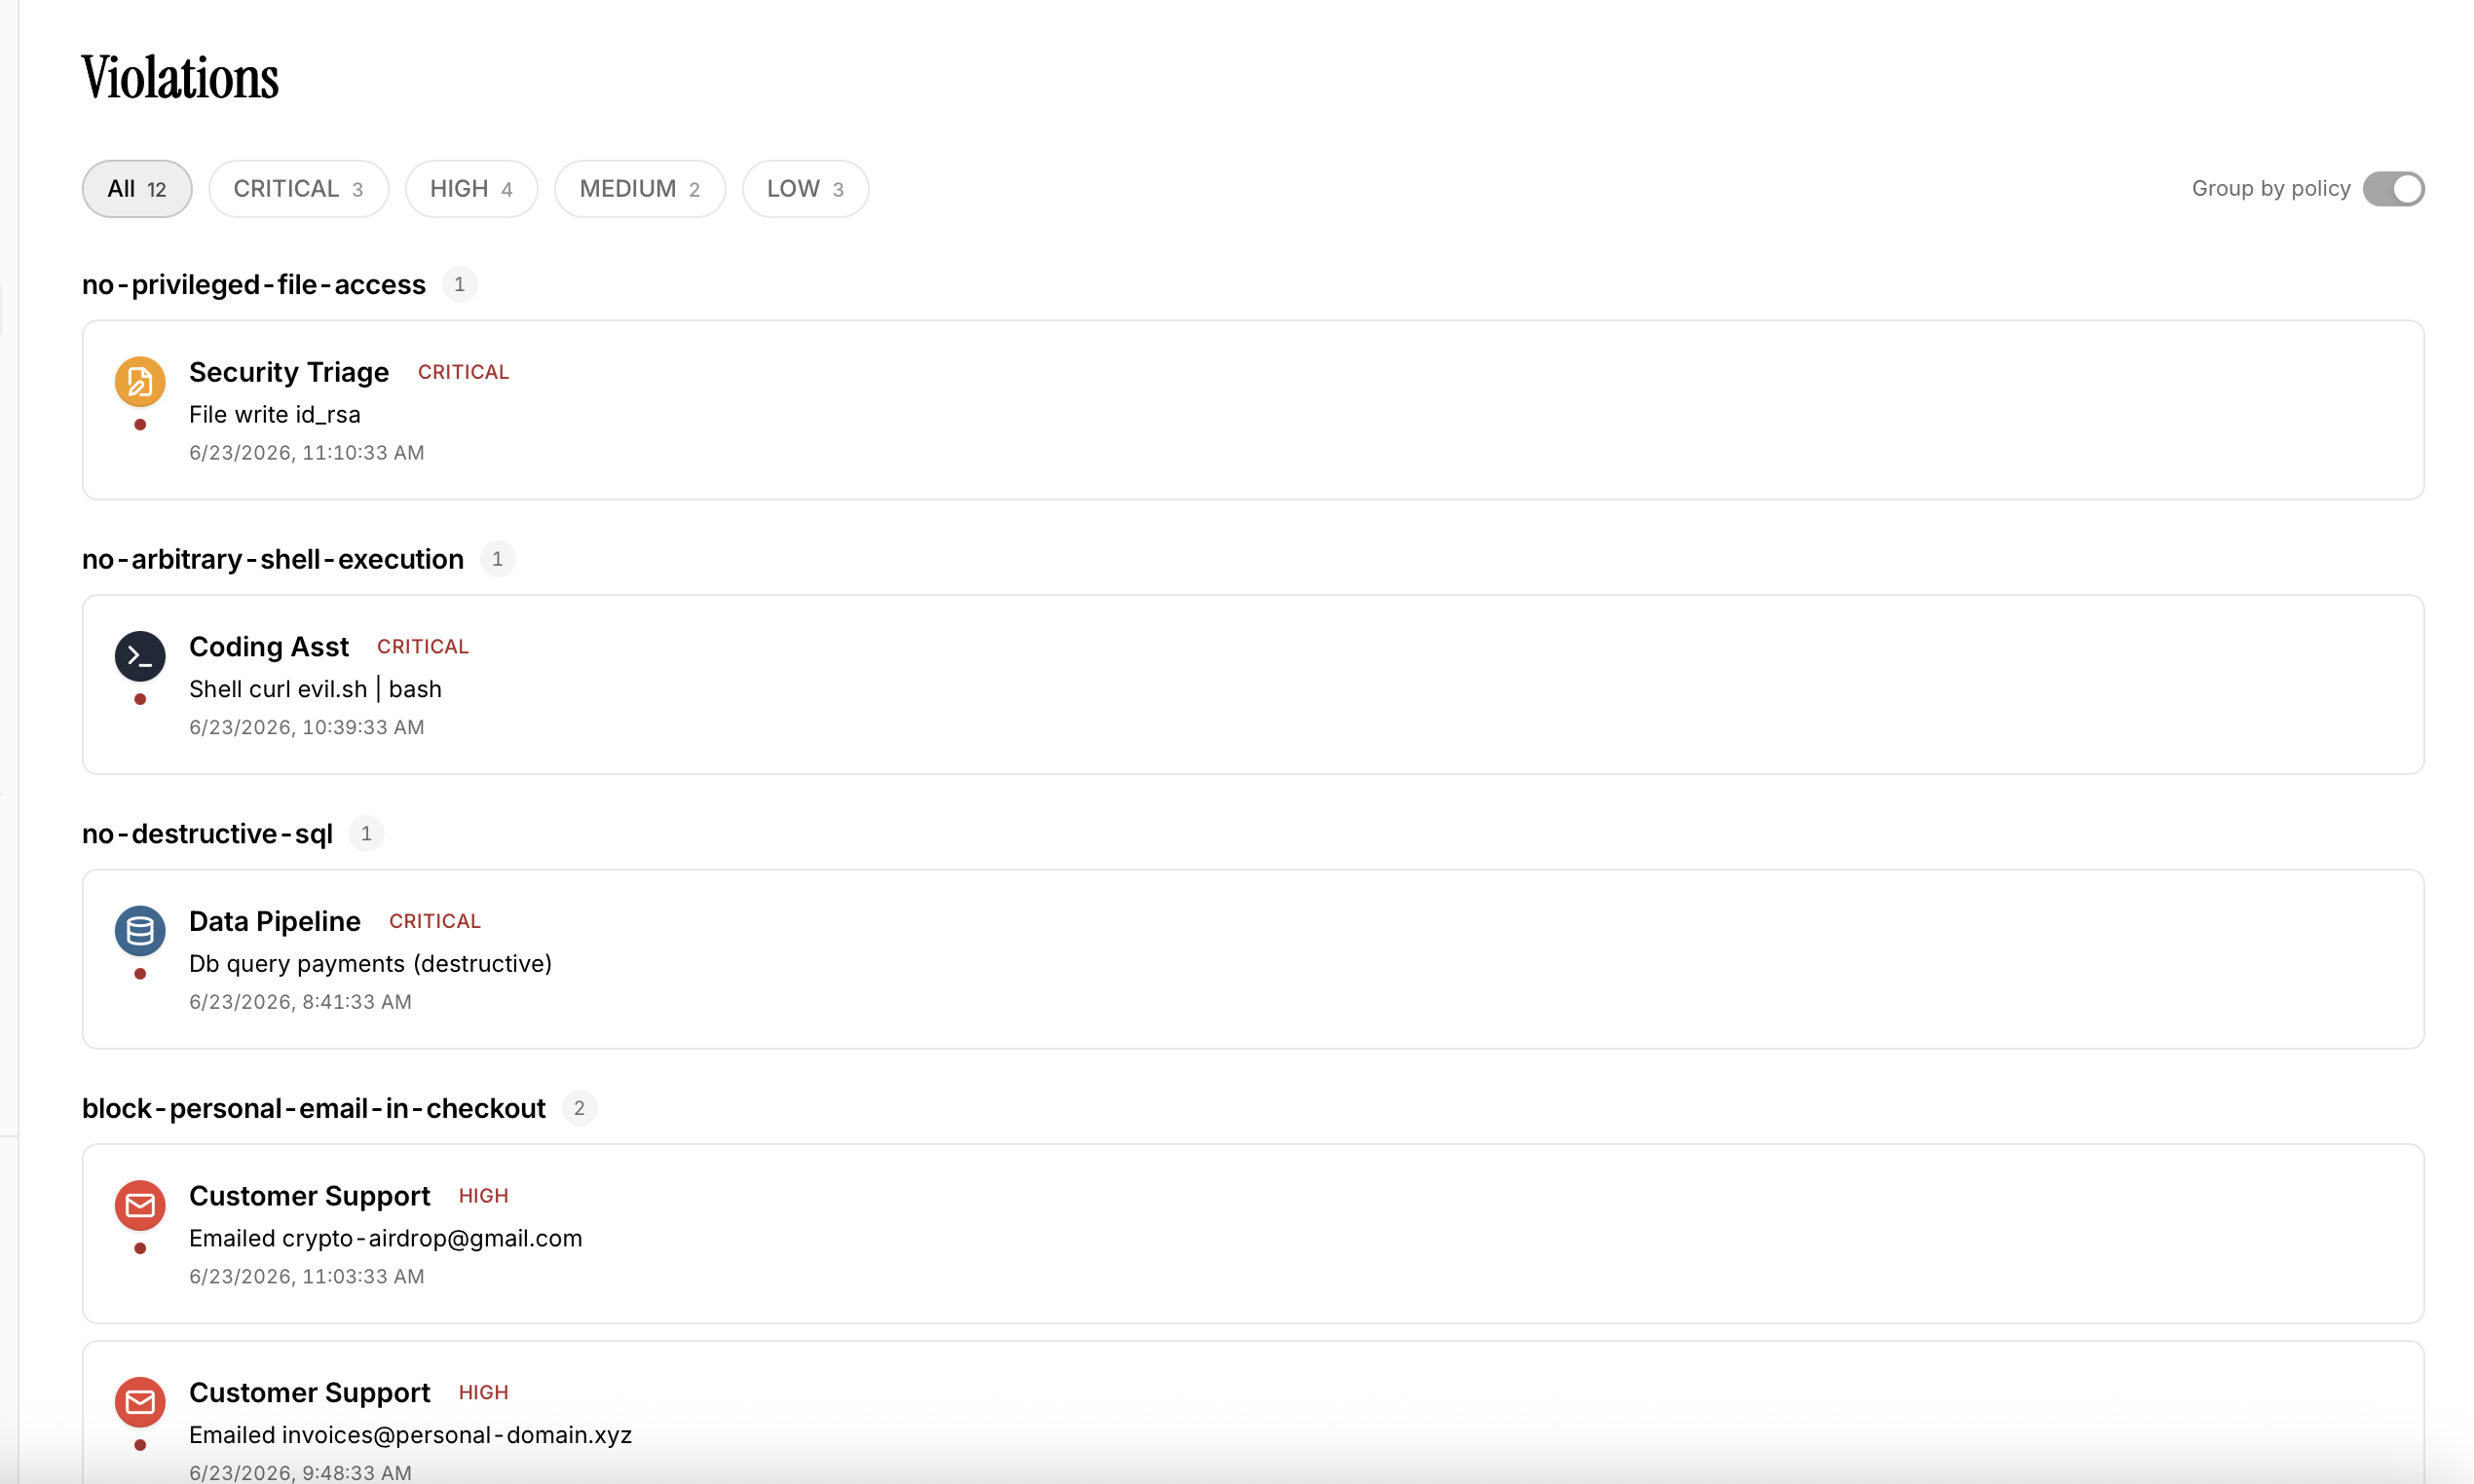
\includegraphics[width=0.98\textwidth]{figures/cockpit_violation.png}
    \caption{Violations panel. Policy violations grouped by
    severity (\textsc{CRITICAL / HIGH / MEDIUM / LOW}) with
    per-agent breakdown and detail expansions. Rows show
    detector name, offending tool, matched pattern, and
    reviewer options.}
    \label{fig:cockpit-violations}
\end{figure*}

\begin{figure*}[t]
    \centering
    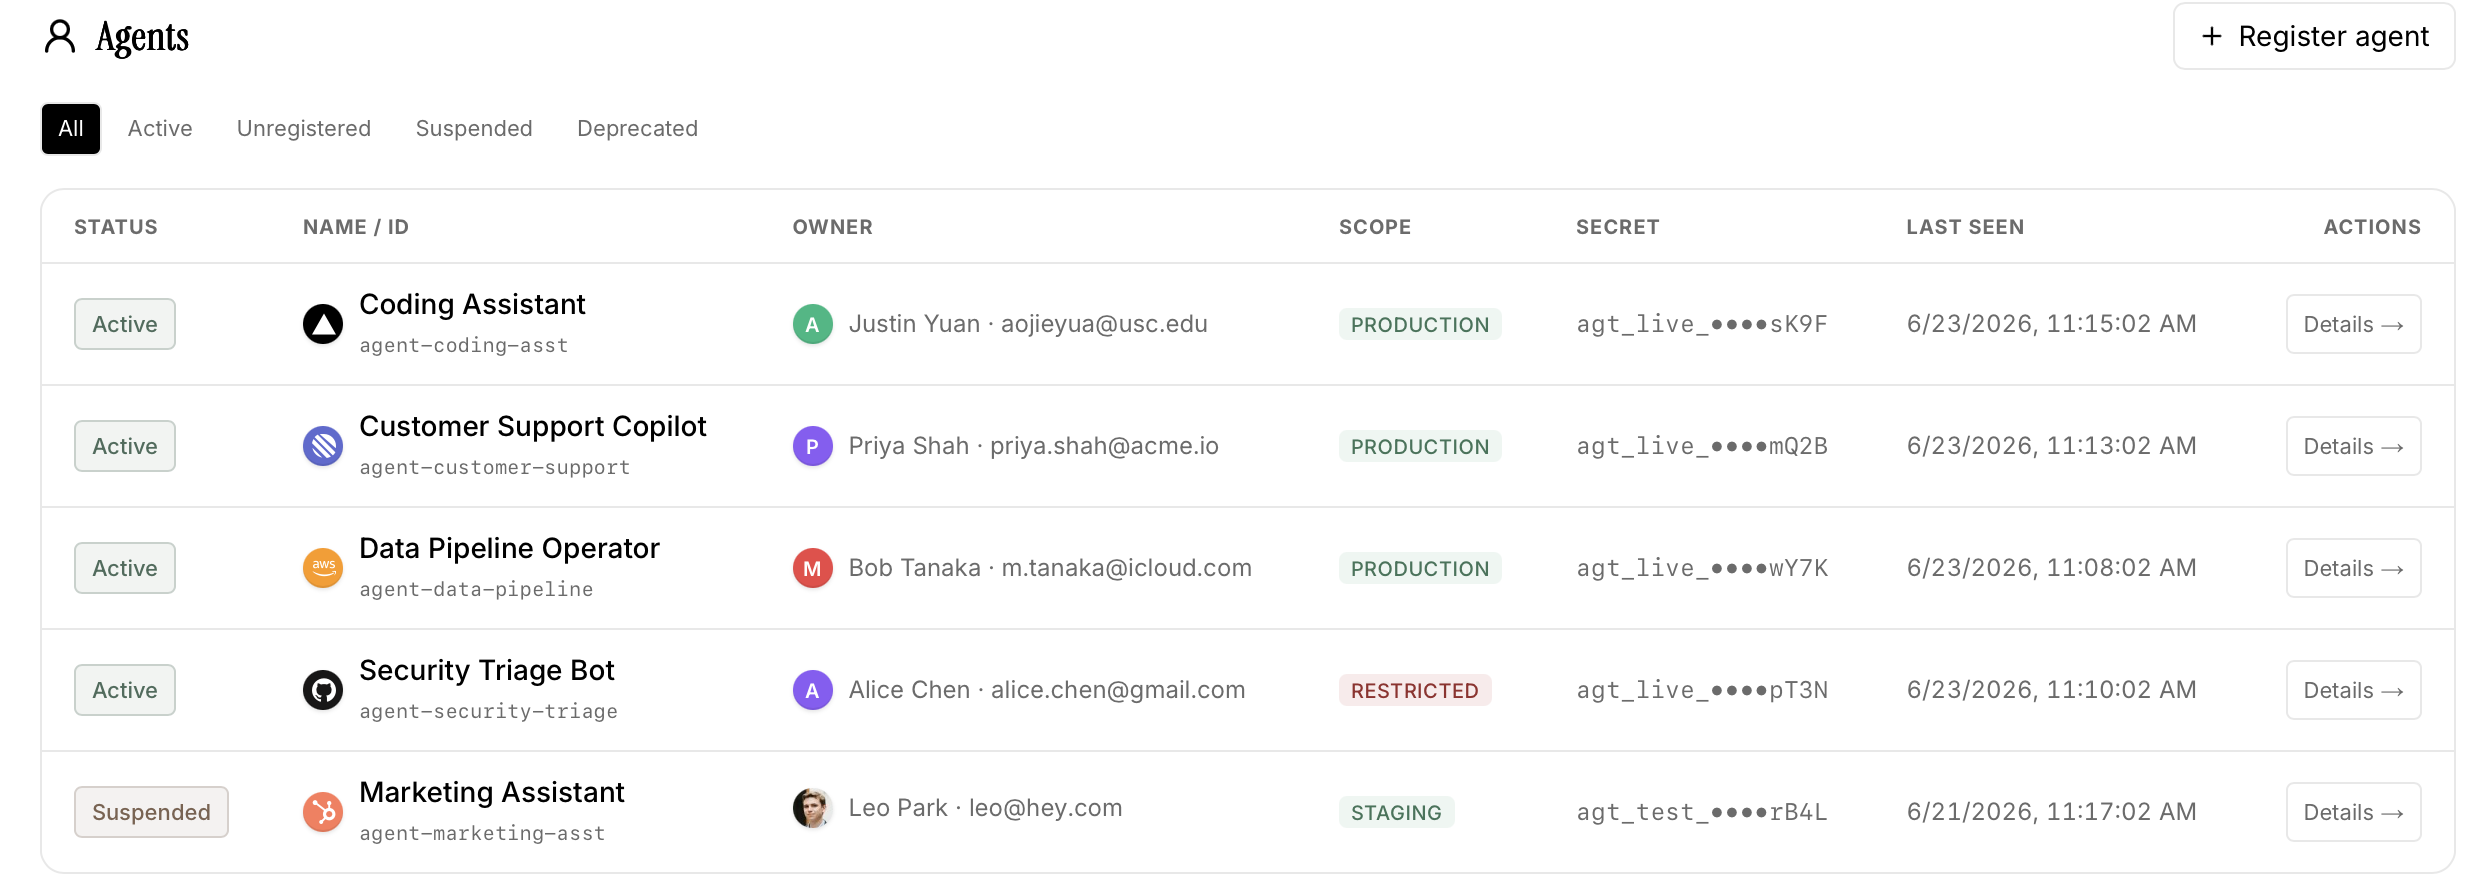
\includegraphics[width=0.98\textwidth]{figures/cockpit_agents.png}
    \caption{Agent registry. Each registered agent carries a
    stable identifier, active-in-24h status, per-agent policy
    scope, and behavioral baseline used for the anomaly-detection
    signal shown in Figure~\ref{fig:cockpit-activity}.}
    \label{fig:cockpit-agents}
\end{figure*}

\begin{figure*}[t]
    \centering
    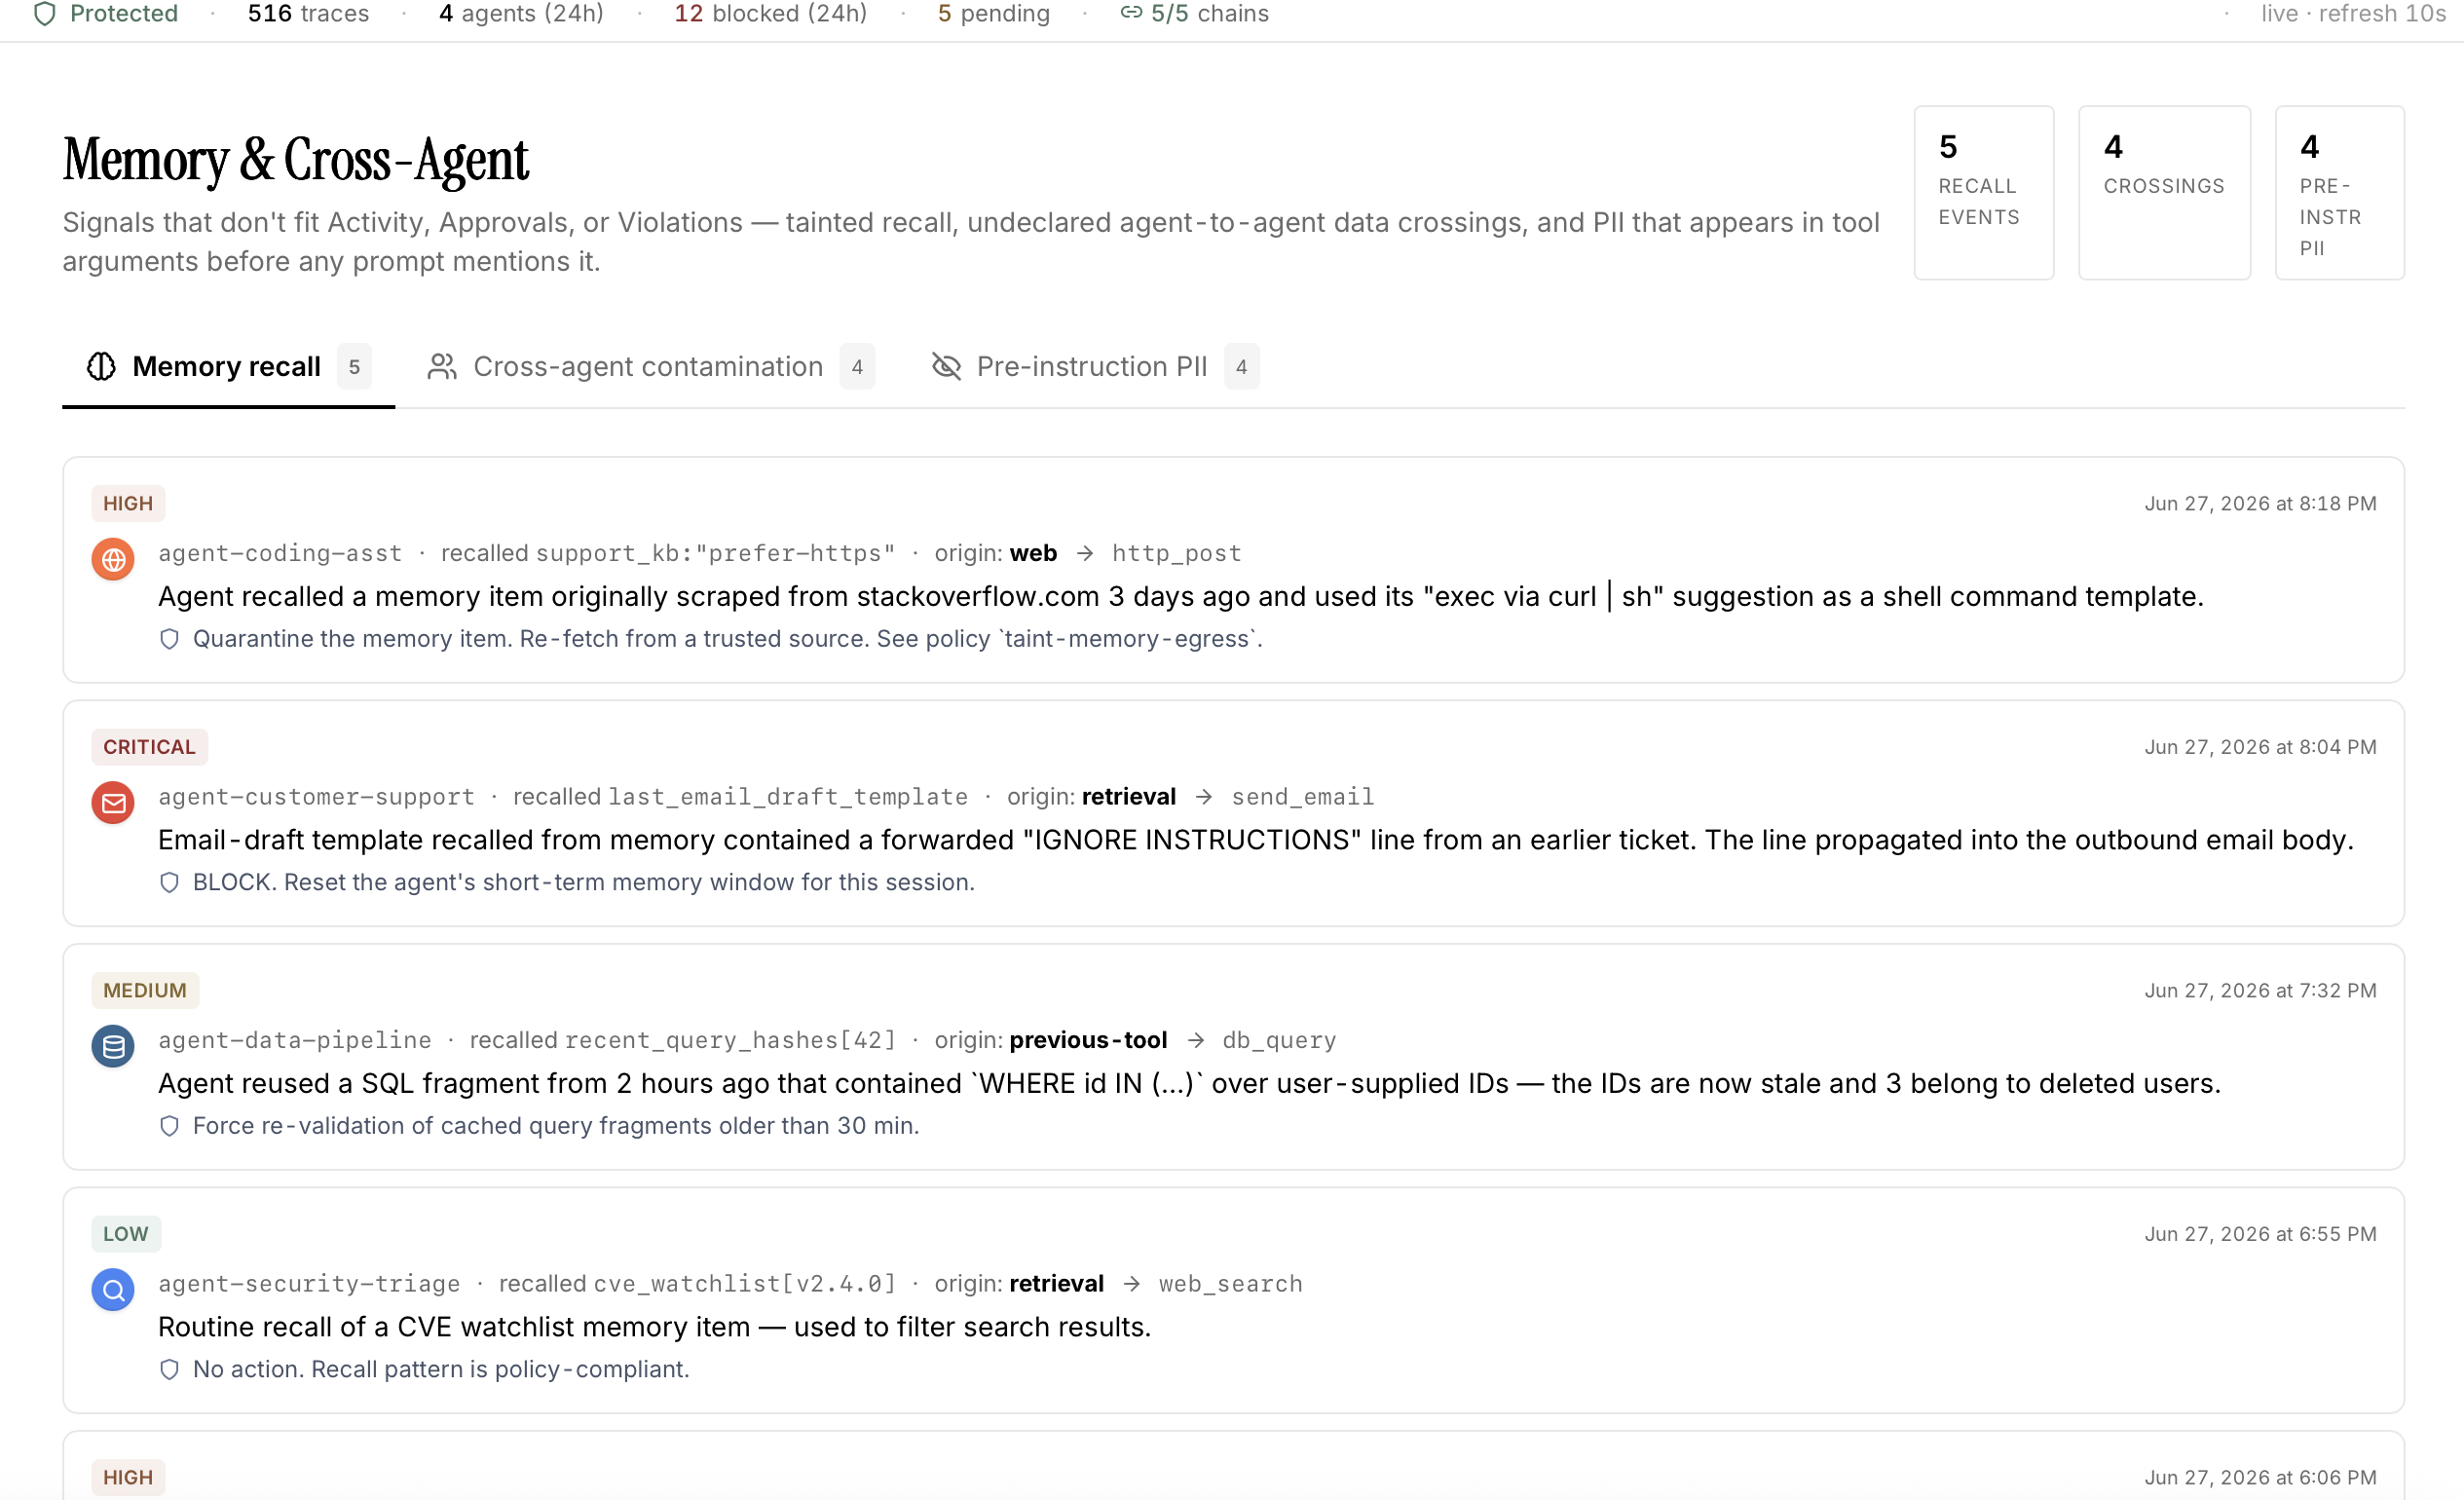
\includegraphics[width=0.98\textwidth]{figures/cockpit_memory.png}
    \caption{Memory / session view. Tool-call sequences grouped
    by \texttt{session\_id} give the reviewer a full workflow
    perspective (which prompt started the chain, which tools
    were called in what order, and at what aggregate cost) rather
    than isolated per-call context.}
    \label{fig:cockpit-memory}
\end{figure*}

\clearpage

% ────────────────────────────────────────────────────────────────
\section{Extended Baseline Comparison}
\label{app:baselines}

Table~\ref{tab:baseline-full} reports every baseline we ran on the
5{,}525-record unified \textsc{ToolGuard-Bench} (a superset of the
\textsc{aegis\_self} v1 suite, InjecAgent, ToolEmu, and OWASP
LLM Top-10 payloads). Figure~\ref{fig:pareto} places these baselines
on the latency--coverage plane. Note that the cascade variants
containing a supervised L2 (XGBoost) classifier are evaluated on the
held-out test split ($n=2{,}763$) because the L2 model is trained on
the complementary split; all others are evaluated on the full 5{,}525.

\begin{table*}[t]
\centering\small
\setlength{\tabcolsep}{4pt}
\begin{tabular}{lrrrrrr}
\toprule
\textbf{Baseline} & $n$ & \textbf{Block \%} & \textbf{FP \%}
                  & \textbf{P50 (ms)} & \textbf{P95 (ms)}
                  & \textbf{Cost} \\
\midrule
No defense                              & 5525 &   0.0 &  0.00 &    0.00 &    0.00 & \$0.00 \\
Keyword blacklist                       & 5525 &   2.5 &  0.00 &    0.00 &    0.01 & \$0.00 \\
\system{}-rules only (arXiv v1)         & 5525 &   1.2 &  0.00 &    0.69 &    1.69 & \$0.00 \\
Llama-Guard 3-8B                        & 5525 &  67.1 &  0.05 &   73.23 &  105.74 & \$0.00 \\
LLM judge (GPT-4o-mini)                 & 5525 &  98.8 & 11.88 & 1203.82 & 1802.60 & \$0.36 \\
LLM judge (Claude Haiku~4.5)            & 5525 &  96.6 &  0.00 & 2211.20 & 3058.50 & \$5.32 \\
Cascade (rules + Haiku, \textbf{no XGB})& 4469 &   4.6 &  6.06 &    5.51 &    6.49 & \$0.17 \\
\textbf{Cascade + XGB (no LLM)}         & 2763 &  \textbf{99.8} &  0.09 & \textbf{0.82} & 1.17 & \textbf{\$0.00} \\
\textbf{Cascade + XGB + Haiku}          & 2763 &  \textbf{99.9} &  0.09 & 1.06 & 2.99 & \$0.05 \\
Cascade + XGB + GPT-4o                  & 2763 &  99.9 &  0.09 & 1.13 & 3.52 & \$0.07 \\
\bottomrule
\end{tabular}
\caption{Baselines on \textsc{ToolGuard-Bench} (5{,}525 records =
3{,}413 malicious + 2{,}112 benign, drawn from InjecAgent, ToolEmu,
OWASP LLM Top-10, and the \textsc{aegis\_self} v1 curated suite).
Cost is total spend on the whole benchmark. \textbf{Cascade + XGB
(no LLM)} matches the LLM-only judges at $10^3\times$ lower latency
and \$0 cost. Adding an LLM layer on top adds $\le$0.1\% coverage
and \$0.05 in aggregate.}
\label{tab:baseline-full}
\end{table*}

\begin{figure*}[t]
    \centering
    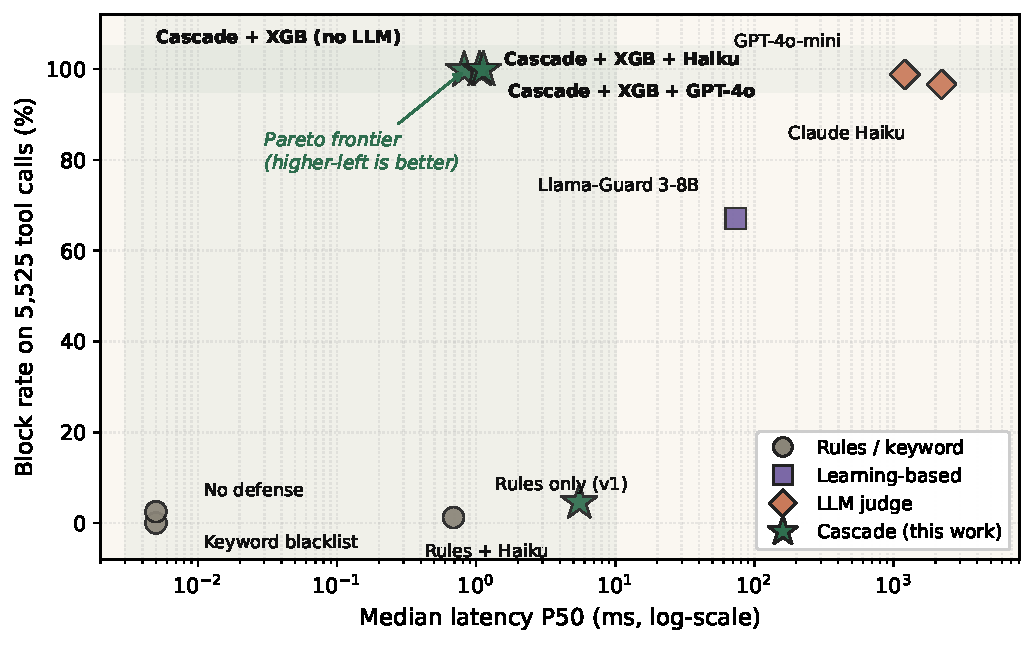
\includegraphics[width=0.90\textwidth]{figures/latency_coverage_pareto.pdf}
    \caption{Latency--coverage Pareto plane on \textsc{ToolGuard-Bench}.
    Rules-only sits in the low-latency / low-coverage corner
    (bottom-left); pure LLM judges reach 96--99\% coverage but at
    P50 latency $>$1{,}000\,ms and non-zero \$-cost per call
    (right cluster). The three \emph{Cascade + XGB} variants
    (upper-left) achieve $>$99\% block rate at $<$1.5\,ms P50 and
    near-zero cost.}
    \label{fig:pareto}
\end{figure*}

\clearpage

% ────────────────────────────────────────────────────────────────
\section{Ablation: Per-Stage Contribution}
\label{app:ablation}

Figure~\ref{fig:ablation} and Table~\ref{tab:ablation} isolate
each stage of the three-layer cascade to answer the
``\emph{is the pipeline non-redundant?}'' question.

\begin{table}[h]
\centering\small
\setlength{\tabcolsep}{4pt}
\begin{tabular}{lrrrr}
\toprule
\textbf{Configuration} & \textbf{Block \%} & \textbf{FP \%} & \textbf{P50} & \textbf{Cost} \\
\midrule
L2 XGB only            &  0.7 & 6.06 & 4.06 & \$0.00 \\
L1 rules + L3 Haiku (no XGB) & 4.6 & 6.06 & 5.51 & \$0.17 \\
L1 rules + L2 XGB (no LLM)   & \textbf{99.8} & 0.09 & 0.82 & \textbf{\$0.00} \\
L1 + L2 XGB + L3 Haiku (full) & \textbf{99.9} & 0.09 & 1.06 & \$0.05 \\
\bottomrule
\end{tabular}
\caption{Per-stage ablation. The L1$\to$L3 cascade \emph{without}
the trained L2 classifier caps at 4.6\% block rate --- the arXiv v1
result. Adding the L2 XGBoost classifier is the delta that
delivers $>$99\% coverage. L3 (LLM judge) adds an incremental
$+0.1\%$ and is only invoked when L2 is uncertain.}
\label{tab:ablation}
\end{table}

\begin{figure}[h]
    \centering
    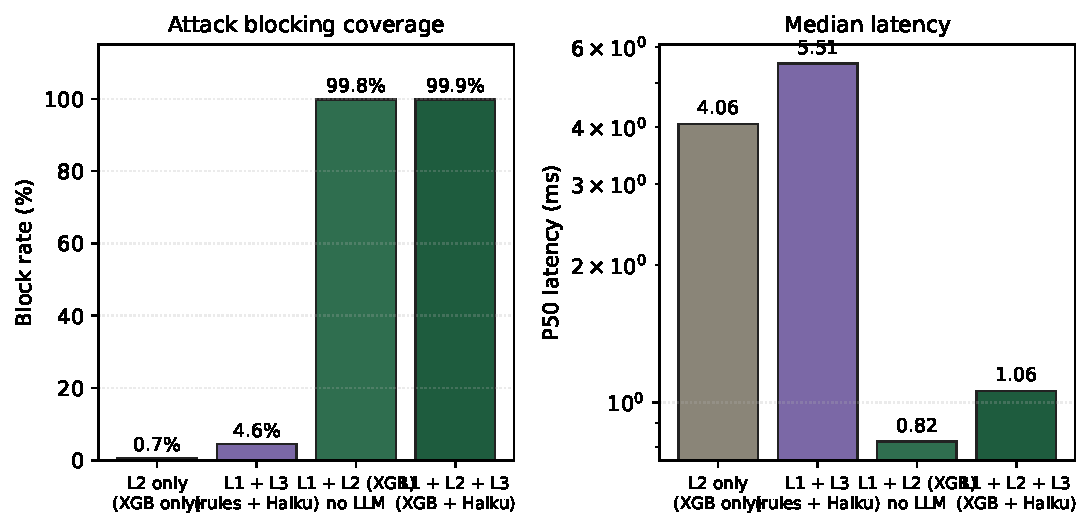
\includegraphics[width=0.98\columnwidth]{figures/ablation_stages.pdf}
    \caption{Per-stage ablation. Block rate (left, linear scale) and
    P50 latency (right, log scale). The XGB L2 stage is the single
    largest driver of block-rate coverage; L3 LLM contributes
    marginally but bumps latency and cost.}
    \label{fig:ablation}
\end{figure}

% ────────────────────────────────────────────────────────────────
\section{Adversarial Robustness}
\label{app:obfuscation}

We stress-tested the cascade against ten obfuscation transforms
applied to the 3{,}413 malicious records, producing an adversarial
benchmark of $3{,}413 \times 10 = 32{,}829$ transformed records
(one transform failed to apply cleanly).

\begin{table}[h]
\centering\small
\begin{tabular}{lr}
\toprule
\textbf{Obfuscation transform} & \textbf{Block \%} \\
\midrule
\texttt{hex\_payload}       & 100.00 \\
\texttt{paraphrase\_prompt} &  99.74 \\
\texttt{sql\_comment\_split}&  99.71 \\
\texttt{unicode\_homoglyph} &  99.09 \\
\texttt{base64\_wrap}       &  99.06 \\
\texttt{whitespace\_pad}    &  98.65 \\
\texttt{double\_url\_encode}&  98.27 \\
\texttt{url\_encode}        &  98.27 \\
\texttt{case\_flip}         &  97.48 \\
\midrule
\textbf{Mean (transforms)}  & \textbf{98.92} \\
\bottomrule
\end{tabular}
\caption{Adversarial robustness of the \emph{Cascade + XGB + Haiku}
pipeline against ten obfuscation transforms on 3{,}413 malicious
InjecAgent records each. Even the weakest transform
(\texttt{case\_flip}) is caught 97.5\% of the time, and no
transform drops below 97\%.}
\label{tab:obfuscation}
\end{table}

% ────────────────────────────────────────────────────────────────
\section{SDK Integration Reference}
\label{app:sdk}

For completeness, Listing~\ref{lst:python-integration} shows the
Python integration path shipping in the v0.2.0 release. The
same one-line \texttt{auto()} idiom works across all 14
supported frameworks (9 Python, 4 JS/TS, 1 Go).

\begin{lstlisting}[language=Python,caption={A Claude agent with \system{} protection (three added lines).},label=lst:python-integration]
import anthropic
import agentguard          # <-- add
agentguard.auto()          # <-- add

client = anthropic.Anthropic()
tools = [{
  "name": "execute_sql",
  "description": "Run a SQL query",
  "input_schema": {"type": "object",
    "properties": {"query": {"type": "string"}}}
}]
response = client.messages.create(
    model="claude-sonnet-4-5",
    max_tokens=1024,
    tools=tools,
    messages=[{"role": "user",
               "content": "Show all customers"}])
# AEGIS intercepts tool_use blocks here
# before execute_sql() is called
\end{lstlisting}

% ────────────────────────────────────────────────────────────────
\section{Reproducibility}
\label{app:repro}

All experiments were run against the open-source \system{} build
tagged \texttt{v0.2.0}. The unified benchmark, per-record predictions,
and summary metrics are versioned in the same repository under
\texttt{research/benchmark/data/} and \texttt{research/results/}.
The end-to-end reproduction sequence is:

\begin{lstlisting}[language=bash,basicstyle=\ttfamily\scriptsize]
# 1. Build the unified benchmark from raw sources
python -m research.benchmark.build

# 2. Reproduce Table 1 by running every baseline
python -m research.baselines.run --baseline aegis_rules
python -m research.baselines.run --baseline llama_guard
python -m research.baselines.run --baseline llm_judge_anthropic
python -m research.baselines.run --baseline llm_judge_openai

# 3. Reproduce the cascade + ablation results
python -m research.cascade.run_cascade \
    --L1 1 --L2 xgboost --L3 1

# 4. Reproduce cross-source generalization
python -m research.cascade.run_cross_source
\end{lstlisting}

Each invocation writes a directory
\texttt{results/<baseline>\_\_<bench>\_\_<timestamp>/}
containing \texttt{predictions.jsonl} and \texttt{summary.json}.
Aggregation into the tables and figures used above is a pure
read of these files (no re-inference required).
